\hypertarget{LinearStatistic_8h}{
\section{LinearStatistic.h File Reference}
\label{LinearStatistic_8h}\index{LinearStatistic.h@{LinearStatistic.h}}
}


This graph shows which files directly or indirectly include this file:\nopagebreak
\begin{figure}[H]
\begin{center}
\leavevmode
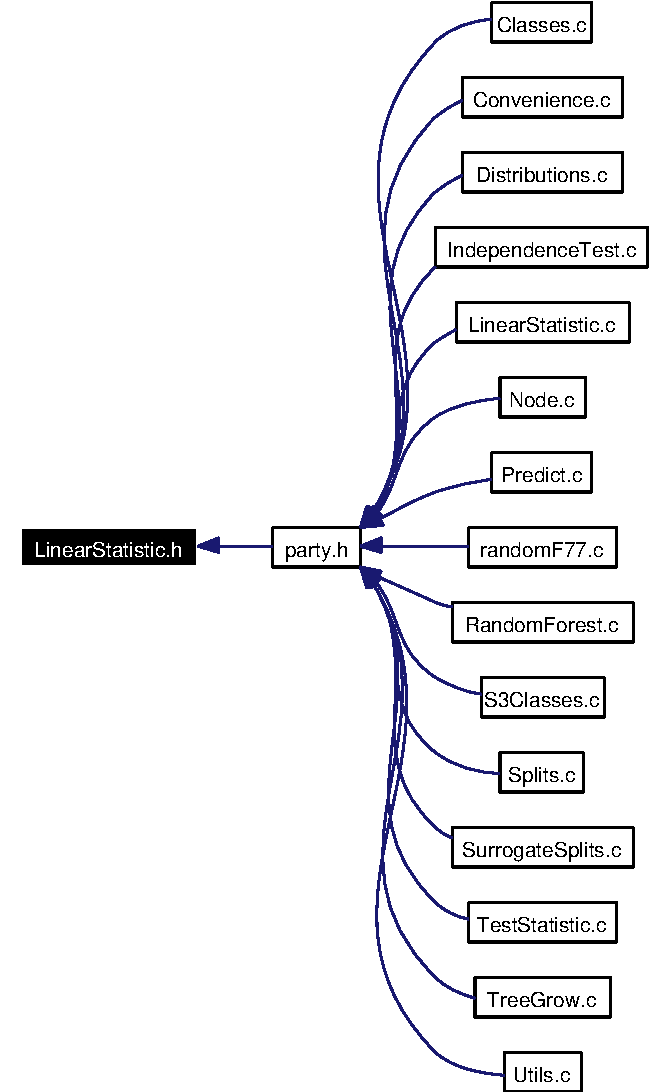
\includegraphics[width=420pt]{LinearStatistic_8h__dep__incl}
\end{center}
\end{figure}
\subsection*{Functions}
\begin{CompactItemize}
\item 
void \hyperlink{LinearStatistic_8h_aefa2a9406bb30b323715e3db41da637}{C\_\-LinearStatistic} (const double $\ast$x, const int p, const double $\ast$y, const int q, const double $\ast$weights, const int n, double $\ast$ans)
\item 
void \hyperlink{LinearStatistic_8h_e2f62abe13ee5b625141b5d4a496d832}{C\_\-ExpectCovarInfluence} (const double $\ast$y, const int q, const double $\ast$weights, const int n, SEXP ans)
\item 
void \hyperlink{LinearStatistic_8h_94a0805ea258af79d426c095feee399a}{C\_\-ExpectCovarLinearStatistic} (const double $\ast$x, const int p, const double $\ast$y, const int q, const double $\ast$weights, const int n, const SEXP expcovinf, SEXP ans)
\item 
void \hyperlink{LinearStatistic_8h_a34b0f12fac36231a105d6dc903bfe89}{C\_\-PermutedLinearStatistic} (const double $\ast$x, const int p, const double $\ast$y, const int q, const int n, const int nperm, const int $\ast$indx, const int $\ast$perm, double $\ast$ans)
\item 
SEXP \hyperlink{LinearStatistic_8h_6216ea560644c08002fb32756ae67dcc}{R\_\-ExpectCovarInfluence} (SEXP y, SEXP weights)
\end{CompactItemize}


\subsection{Function Documentation}
\hypertarget{LinearStatistic_8h_e2f62abe13ee5b625141b5d4a496d832}{
\index{LinearStatistic.h@{LinearStatistic.h}!C_ExpectCovarInfluence@{C\_\-ExpectCovarInfluence}}
\index{C_ExpectCovarInfluence@{C\_\-ExpectCovarInfluence}!LinearStatistic.h@{LinearStatistic.h}}
\subsubsection{\setlength{\rightskip}{0pt plus 5cm}void C\_\-ExpectCovarInfluence (const double $\ast$ {\em y}, const int {\em q}, const double $\ast$ {\em weights}, const int {\em n}, SEXP {\em ans})}}
\label{LinearStatistic_8h_e2f62abe13ee5b625141b5d4a496d832}


Conditional expectation and covariance of the influence function\par
 \begin{Desc}
\item[Parameters:]
\begin{description}
\item[{\em y}]values of the influence function \item[{\em q}]dimension of the influence function \item[{\em weights}]case weights \item[{\em n}]number of observations \item[{\em ans}]return value; an object of class `ExpectCovarInfluence' \end{description}
\end{Desc}


Definition at line 101 of file LinearStatistic.c.

References PL2\_\-covarianceSym, PL2\_\-expectationSym, and PL2\_\-sumweightsSym.\hypertarget{LinearStatistic_8h_94a0805ea258af79d426c095feee399a}{
\index{LinearStatistic.h@{LinearStatistic.h}!C_ExpectCovarLinearStatistic@{C\_\-ExpectCovarLinearStatistic}}
\index{C_ExpectCovarLinearStatistic@{C\_\-ExpectCovarLinearStatistic}!LinearStatistic.h@{LinearStatistic.h}}
\subsubsection{\setlength{\rightskip}{0pt plus 5cm}void C\_\-ExpectCovarLinearStatistic (const double $\ast$ {\em x}, const int {\em p}, const double $\ast$ {\em y}, const int {\em q}, const double $\ast$ {\em weights}, const int {\em n}, const SEXP {\em expcovinf}, SEXP {\em ans})}}
\label{LinearStatistic_8h_94a0805ea258af79d426c095feee399a}


Conditional expectation and covariance of the a linear statistic\par
 \begin{Desc}
\item[Parameters:]
\begin{description}
\item[{\em x}]values of the transformation \item[{\em p}]dimension of the transformation \item[{\em y}]values of the influence function \item[{\em q}]dimension of the influence function \item[{\em weights}]case weights \item[{\em n}]number of observations \item[{\em expcovinf}]an object of class `ExpectCovarInfluence' \item[{\em ans}]return value; an object of class `ExpectCovar' \end{description}
\end{Desc}


Definition at line 213 of file LinearStatistic.c.

References C\_\-kronecker(), PL2\_\-covarianceSym, PL2\_\-expectationSym, and PL2\_\-sumweightsSym.

Here is the call graph for this function:\nopagebreak
\begin{figure}[H]
\begin{center}
\leavevmode
\includegraphics[width=159pt]{LinearStatistic_8h_94a0805ea258af79d426c095feee399a_cgraph}
\end{center}
\end{figure}
\hypertarget{LinearStatistic_8h_aefa2a9406bb30b323715e3db41da637}{
\index{LinearStatistic.h@{LinearStatistic.h}!C_LinearStatistic@{C\_\-LinearStatistic}}
\index{C_LinearStatistic@{C\_\-LinearStatistic}!LinearStatistic.h@{LinearStatistic.h}}
\subsubsection{\setlength{\rightskip}{0pt plus 5cm}void C\_\-LinearStatistic (const double $\ast$ {\em x}, const int {\em p}, const double $\ast$ {\em y}, const int {\em q}, const double $\ast$ {\em weights}, const int {\em n}, double $\ast$ {\em ans})}}
\label{LinearStatistic_8h_aefa2a9406bb30b323715e3db41da637}


Computes the linear statistic, formula (1) in the paper\par
 \begin{Desc}
\item[Parameters:]
\begin{description}
\item[{\em x}]values of the transformation \item[{\em p}]dimension of the transformation \item[{\em y}]values of the influence function \item[{\em q}]dimension of the influence function \item[{\em weights}]case weights \item[{\em n}]number of observations \item[{\em ans}]return value; a pointer to a REALSXP-vector of length pq \end{description}
\end{Desc}


Definition at line 23 of file LinearStatistic.c.\hypertarget{LinearStatistic_8h_a34b0f12fac36231a105d6dc903bfe89}{
\index{LinearStatistic.h@{LinearStatistic.h}!C_PermutedLinearStatistic@{C\_\-PermutedLinearStatistic}}
\index{C_PermutedLinearStatistic@{C\_\-PermutedLinearStatistic}!LinearStatistic.h@{LinearStatistic.h}}
\subsubsection{\setlength{\rightskip}{0pt plus 5cm}void C\_\-PermutedLinearStatistic (const double $\ast$ {\em x}, const int {\em p}, const double $\ast$ {\em y}, const int {\em q}, const int {\em n}, const int {\em nperm}, const int $\ast$ {\em indx}, const int $\ast$ {\em perm}, double $\ast$ {\em ans})}}
\label{LinearStatistic_8h_a34b0f12fac36231a105d6dc903bfe89}


Linear Statistic with permuted indices\par
 \begin{Desc}
\item[Parameters:]
\begin{description}
\item[{\em x}]values of the transformation \item[{\em p}]dimension of the transformation \item[{\em y}]values of the influence function \item[{\em q}]dimension of the influence function \item[{\em n}]number of observations \item[{\em nperm}]number of permutations \item[{\em indx}]indices for the x-part \item[{\em perm}](permuted) indices for the y-part \item[{\em ans}]return value; a pointer to a REALSXP-vector of length pq \end{description}
\end{Desc}


Definition at line 351 of file LinearStatistic.c.\hypertarget{LinearStatistic_8h_6216ea560644c08002fb32756ae67dcc}{
\index{LinearStatistic.h@{LinearStatistic.h}!R_ExpectCovarInfluence@{R\_\-ExpectCovarInfluence}}
\index{R_ExpectCovarInfluence@{R\_\-ExpectCovarInfluence}!LinearStatistic.h@{LinearStatistic.h}}
\subsubsection{\setlength{\rightskip}{0pt plus 5cm}SEXP R\_\-ExpectCovarInfluence (SEXP {\em y}, SEXP {\em weights})}}
\label{LinearStatistic_8h_6216ea560644c08002fb32756ae67dcc}


R-interface to C\_\-ExpectCovarInfluence\par
 \begin{Desc}
\item[Parameters:]
\begin{description}
\item[{\em y}]values of the influence function \item[{\em weights}]case weights \end{description}
\end{Desc}


Definition at line 171 of file LinearStatistic.c.

References C\_\-ExpectCovarInfluence(), ncol(), nrow(), PL2\_\-covarianceSym, PL2\_\-expectationSym, and PL2\_\-sumweightsSym.

Here is the call graph for this function:\nopagebreak
\begin{figure}[H]
\begin{center}
\leavevmode
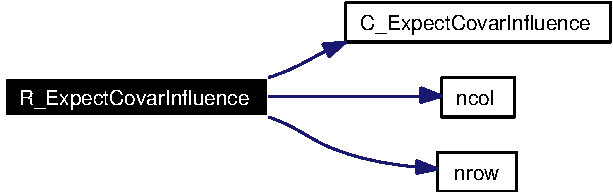
\includegraphics[width=177pt]{LinearStatistic_8h_6216ea560644c08002fb32756ae67dcc_cgraph}
\end{center}
\end{figure}
